%% Using LaTeX-Boilerplate by Adrian-Tudor Panescu %%
%% https://github.com/adrianp/latex-boilerplate %%

\documentclass[12pt,a4paper,twoside]{report}

\def\pdfshellescape{1} % for epstopdf


\usepackage[utf8]{inputenc}
\usepackage[british]{babel}

\usepackage{algorithm}  % in texlive-science
\usepackage{algorithmic}
\usepackage{amsfonts}
\usepackage{amsmath}
\usepackage{amssymb}
\usepackage{appendix}
\usepackage{caption}
\usepackage{listings}
\usepackage[left=2cm,right=2cm,top=2cm,bottom=2cm]{geometry}
\usepackage{graphicx}
\usepackage{hyperref}
\usepackage{makeidx}
\usepackage{placeins}
\usepackage{subcaption}

\usepackage{epstopdf}  % load after graphic[s,x]


%% bold float labels
\DeclareCaptionLabelFormat{myformat}{\textbf{#1}~\textbf{#2}}
\captionsetup{labelformat=myformat}

%% detailled margin sizes
%\addtolength{\textwidth}{4cm}
%\addtolength{\oddsidemargin}{-1.5cm}
%\addtolength{\evensidemargin}{-1.5cm}
%\addtolength{\textheight}{4.5cm}
%\addtolength{\topmargin}{-3cm}
%\setlength{\parindent}{0pt}
%\setlength{\parskip}{1ex}

%% Section number format
\renewcommand*\thesection{\arabic{section}}

%% Give numbers to subsubsections and add them to index
\setcounter{secnumdepth}{3}
\setcounter{tocdepth}{3}

% rename abstract with care for babel package
\addto\captionsbritish{%
  \renewcommand{\abstractname}%
  {Summary}%
}

%% rename index with care for babel package
\addto\captionsbritish{%
  \renewcommand{\contentsname}%
  {Table of Contents}%
}

%% special table cell that allows line breaks
\newcommand{\specialcell}[2][l]{%
  \begin{tabular}[#1]{@{}c@{}}#2\end{tabular}}

%% do not split long footnotes over multiple pages
\interfootnotelinepenalty=10000


\author{
    Adrian-Tudor Panescu \\
    \href{mailto:adrian@panescu.com}{adrian@panescu.com}
  \and
    John Doe
}
\title{LaTeX Boilerplate}
\date{}  % no date


\begin{document}

  %!TEX root=../main.tex

\maketitle


  % blank pages are inserted for two-side printing
  %!TEX root=../main.tex

\thispagestyle{empty}
%\addtocounter{page}{-1} % do not count this page
\newpage
\mbox{}
\pagebreak


  \setcounter{page}{3}

  \begin{abstract}
    %!TEX root=../main.tex

This project aims at enhancing the scientific user community features related
to shared commenting and annotating of scientific literature and data
resources.  The current commenting practices in digital repositories often
cover global, per-document commenting options only. Within the Large Hadron
Collider experiment collaborations at CERN, more targeted needs include
per-section, per-line, or per data item commenting granularity.

In the context of Invenio, a digital library platform originating in the
high-energy physics community, a framework which allows annotating various
types of data resources has been developed. By leveraging it, a general Web
page annotator, and a targeted document commenting system, which allows
referring to specific elements such as pages, sections, figures, or
mathematical equations have been delivered.

State of the art technologies have been employed in order to deliver solutions
which are in line with current Web application practices. The framework
includes an annotation dissemination mechanism, which adheres to standards such
as JSON-LD and REST services, and emerging specifications such as the Open
Annotation RDF data model.

  \end{abstract}

  \tableofcontents
  \listoffigures
  \listoftables
  \lstlistoflistings

  % next page will be odd-numbered (assumes \FloatBarrier)
  \cleardoublepage

  \section{Introduction}
    \label{sec:intro}
    %!TEX root=../../main.tex

\paragraph{Thesis Structure} The next section provides an overview on the state
of the art of various commenting and annotating systems, as well as on a number
of technologies for linking data on the Web. Section \ref{sec:design} describes
the conceptual design of the system, and also provides a short account of the
changes scheduled for the next Invenio version, to which this project brought a
number of contributions. Section \ref{sec:impl} details the implementation
aspects and technologies of the annotation solution. The thesis ends with a
number of conclusions and future work possibilities.


  \cleardoublepage

  \section{Examples}
    \label{sec:ex}
    This section exemplifies some useful elements.

    \FloatBarrier

    \subsection{Algorithm}
      \label{sec:algo}
      %!TEX root=../../main.tex

This section exeplifies an algorithm environment \ref{alg:fizz} and
a\footnote{footnote}.

\begin{algorithm}{$FizzBuzz(n)$}
  \caption{FizzBuzz}
  \label{alg:fizz}
  \begin{algorithmic}[2]
    \FOR{$i \gets 1; i \le n; i \gets i+1$}
      \IF{$i$ is divisible by $15$}
        \STATE{output FizzBuzz}
      \ELSIF{$i$ is divisible by $3$}
        \STATE{output Fizz}
      \ELSIF{$i$ is divisible by $5$}
        \STATE{output Buzz}
      \ELSE
        \STATE{output i}
      \ENDIF
    \ENDFOR
  \end{algorithmic}
\end{algorithm}


    \clearpage

    \subsection{Listing}
      \label{sec:lst}
      %!TEX root=../../main.tex

This sections exemplifies a source code listing \ref{lst:lst}.

\vspace*{1\baselineskip}

\lstinputlisting[language=Python,
                 caption=Python 3 implementation of the Fizz Buzz game,
                 label=lst:lst,
                 frame=tb,
                 captionpos=b,
                 numbers=left,
                 showspaces=false,
                 showstringspaces=false,
                 showtabs=false,
                 stepnumber=2,
                 numbersep=4pt]
  {static/lst/fizzbuzz.py}


    \clearpage

    \subsection{Float}
      \label{sec:float}
      %!TEX root=../../main.tex

This section demonstrates how to insert images in your document.


      \FloatBarrier

      \subsubsection{Figure}
        \label{sec:fig}
        %!TEX root=../../main.tex

Here is an example of a Figure \ref{fig:fig}.

\begin{figure}[!h]
  \centering
  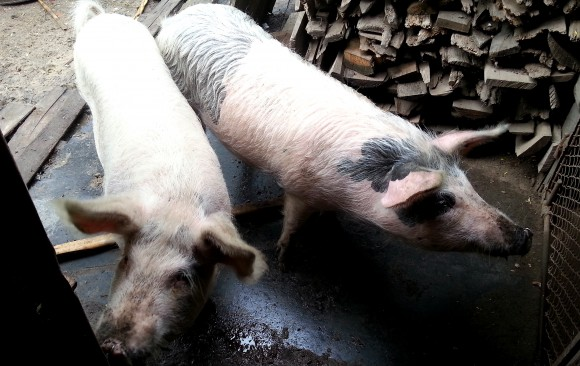
\includegraphics[scale=0.5]{static/img/pigs1.jpg}
  \caption{Pigs, pigs, pigs.}
  \label{fig:fig}
\end{figure}


      \FloatBarrier

      \subsubsection{Subfigure}
        \label{sec:subfig}
        %!TEX root=../../main.tex

And here is an example of a float \ref{fig:subex} with subfigures
\ref{fig:subex:pigs} and \ref{fig:subex:pig}.

\begin{figure}[!h]
  \centering
  \begin{subfigure}[b]{0.3\textwidth}
    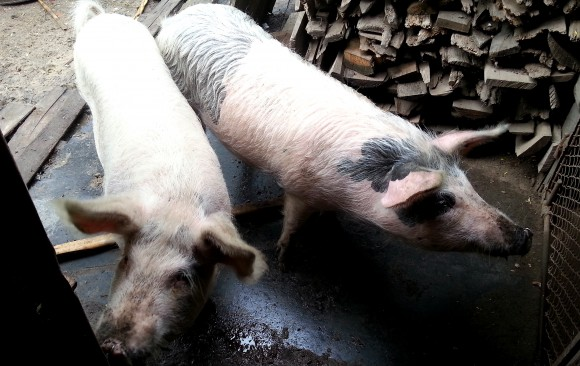
\includegraphics[width=\textwidth]{static/img/pigs1.jpg}
    \caption{Some pigs.}
    \label{fig:subex:pigs}
  \end{subfigure}
  \begin{subfigure}[b]{0.3\textwidth}
    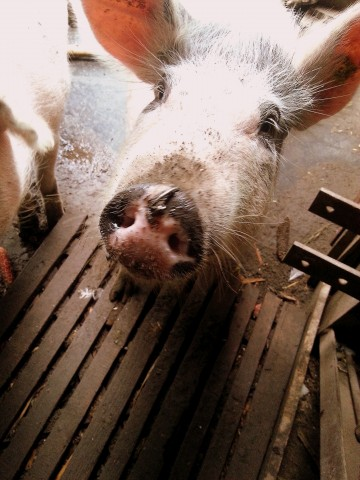
\includegraphics[width=\textwidth]{static/img/pigs2.jpg}
    \caption{A pig.}
    \label{fig:subex:pig}
  \end{subfigure}
  \caption{Some pigs being pigs.}
  \label{fig:subex}
\end{figure}


     \clearpage

    \subsection{Table}
      \label{sec:tbl}
      %!TEX root=../../main.tex

This section exemplifies insertion of tabular data \ref{tbl:tbl}.

\begin{table}[h]
  \centering
  \begin{tabular}{| c | c | c | c | c |}
    \hline
    \textbf{Value} & \textbf{Fizz} & \textbf{Buzz} & \specialcell[t]{\textbf{Fizz} \\ \textbf{Buzz}} \\ \hline \hline
    1 & No & No & No \\ \hline
    2 & No & No & No \\ \hline
    3 & Yes & No & No \\ \hline
    4 & No & No & No \\ \hline
    5 & No & Yes & No \\ \hline
    6 & Yes & No & No \\ \hline
    7 & No & No & No \\ \hline
    8 & No & No & No \\ \hline
    9 & Yes & No & No \\ \hline
    10 & No & Yes & No \\ \hline
    11 & No & No & No \\ \hline
    12 & Yes & No & No \\ \hline
    13 & No & No & No \\ \hline
    14 & No & No & No \\ \hline
    15 & Yes & Yes & Yes \\ \hline
  \end{tabular}
  \caption{The FizzBuzz game values.}
  \label{tbl:tbl}
\end{table}


  \cleardoublepage

  \section{Conclusions}
    \label{sec:outro}
    %!TEX root=../../main.tex

FIXME: wiki usecases, XTiger form, note validator (hierarchy, syntax), import
annotations from other (web)apps (e.g., Adobe)
FIXME: add annos by REST


  \nocite{*}  % include uncited references
  \bibliographystyle{plain}
  \bibliography{bib/myrefs}

  \appendixpage
  \addappheadtotoc

  \appendix
    \section{An appendix}
    \label{sec:app}
    %!TEX root=../../main.tex

Lorem ipsum dolor sit amet, consectetur adipiscing elit. Vestibulum
nec nisi non dui accumsan dignissim eu in lacus. Pellentesque vel
enim dolor. Mauris condimentum velit dolor, a ultrices purus commodo
in. Etiam malesuada justo libero, vel accumsan est commodo in. Donec
eleifend risus non massa dapibus, sit amet bibendum nibh viverra.
Duis non quam vehicula, fringilla nisi ut, interdum libero. Etiam vel
neque aliquam, suscipit enim ut, laoreet leo.

Aliquam erat volutpat. Cras in lorem mauris. Nunc vel sapien
pharetra, sollicitudin est vitae, auctor ligula. Sed sagittis rutrum
feugiat. Nulla semper, urna sit amet feugiat tincidunt, mauris tellus
egestas dolor, et tempor odio nibh sit amet diam. Quisque eget
ullamcorper odio, in imperdiet nisi. Curabitur varius at libero nec
sollicitudin.

Donec sed est ac lacus lobortis sollicitudin. Morbi dui mi, suscipit
eget pretium sit amet, sollicitudin consectetur purus. Quisque
tincidunt ornare tellus, id tincidunt quam euismod nec. Sed rutrum
mauris non lorem elementum porttitor. Quisque dignissim et diam sit
amet convallis. Nulla sed tellus lobortis sapien tincidunt bibendum.
Phasellus cursus mi diam, vel vestibulum urna consequat eu.
Pellentesque vestibulum, risus a tincidunt pulvinar, tellus mi
vestibulum nulla, non cursus lectus eros ac mi. Duis sollicitudin
mauris massa, malesuada posuere diam tincidunt et. Pellentesque
volutpat ligula sed dolor auctor, nec volutpat enim suscipit. Duis a
metus magna. Vestibulum id turpis ac urna dictum lobortis. Cras
semper sem nec sem dapibus sodales.

Pellentesque convallis a tortor nec tempus. Donec nec varius lectus.
Quisque vel rhoncus nulla, nec ultricies purus. Nulla eget velit
diam. Sed eu sapien sed arcu euismod auctor volutpat sit amet sapien.
Aenean orci eros, ultrices et urna quis, consectetur convallis dolor.
Vestibulum ante ipsum primis in faucibus orci luctus et ultrices
posuere cubilia Curae; Nulla lectus dolor, feugiat vel augue non,
molestie posuere odio. Donec placerat elementum lacus, id auctor eros
commodo id. Sed at blandit tellus.

Nulla nibh massa, porttitor quis blandit dignissim, consectetur at
augue. Vestibulum id sagittis ligula, ac consequat diam. Nunc vel
nunc a tortor porttitor tempus eget at elit. Integer lacinia orci at
suscipit suscipit. Mauris vehicula pulvinar lectus, id posuere orci
semper quis. Nullam porta, sem ac luctus consequat, lectus mi
vulputate dui, id egestas ante massa cursus lorem. Cras a dictum
quam, eu scelerisque justo. Donec id mattis tortor. Proin sodales
ligula quis nisi tempor condimentum. Fusce tincidunt mattis justo.
Curabitur sit amet tortor quam. Maecenas dignissim velit at purus
commodo congue non vitae lacus.


\end{document}
